\chapter{2048と強化学習}
\label{chap:rl}
これまでに2048を対象とした強化学習の研究は数多くなされてきた. 
本章では強化学習の概要, および2048に対する強化学習の先行研究について記述する.

\section{強化学習の概要}
\label{sec:rl_general}
まず本節では2048との関係を踏まえつつ, 一般的な強化学習の概要について記述する.
なお本節の内容は全体に文献~\cite{Sutton1998}を参照して書かれた.

\subsection{マルコフ決定過程}
\label{subsec:mdp}
強化学習は与えられた環境において試行錯誤することを通して, 目標を達成するための戦略や意思決定を学習するための手法である.
学習や意思決定を行う主体はエージェントと呼ばれる.
エージェントは離散タイムステップに従って行動を選択し続け, 環境とやり取りを行う.

このような問題設定はマルコフ決定過程~(MDP)~というモデルによって定式化されている.
MDPは以下の$4$つの要素で構成される. 
\begin{itemize}
  \item 状態集合 $\mathcal{S}$
  \item 行動集合 $\mathcal{A}$
  \item 状態遷移関数$p:\mathcal{S} \times \mathcal{A} \times \mathcal{S} \rightarrow [0,1]$
  \item 報酬関数$r:\mathcal{S} \times \mathcal{A} \times \mathcal{S} \rightarrow \mathbb{R}$
\end{itemize}
エージェントはステップ$t$で状態$S_t \in \mathcal{S}$から行動$A_t \in \mathcal{A}$を選択する.
そして確率$p(S_{t+1}|S_t, A_t)$で次の状態$S_{t+1}$に遷移し, $R_{t+1} = r(S_t, A_t, S_{t+1})$を即時報酬として獲得する.
状態遷移関数と報酬関数は環境のダイナミクスと呼ばれることがある. 
図\ref{fig:mdp}にMDPの概念図を示す.
\begin{figure}[h]
  \centering
  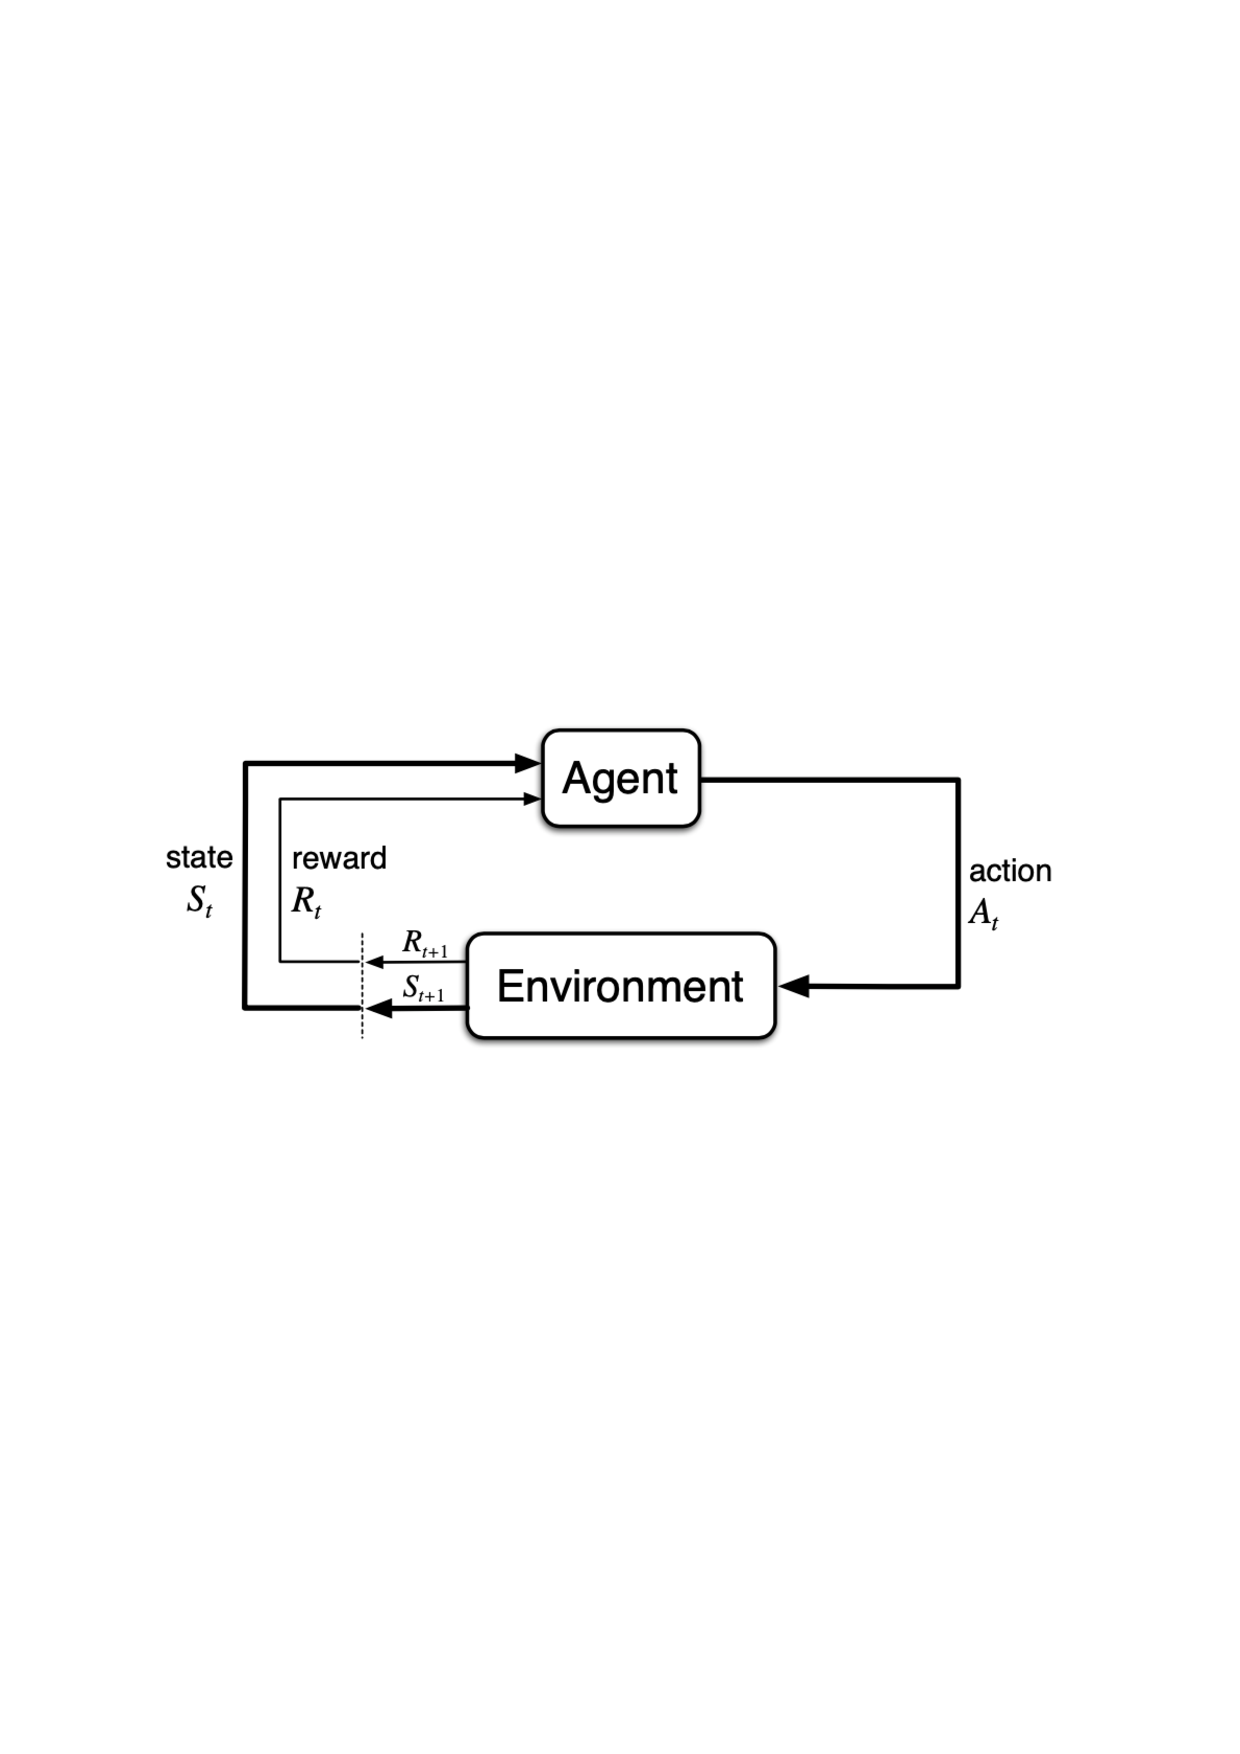
\includegraphics[width=\linewidth{}]{figures/MDP.pdf}
  \caption{MDPの模式図 (文献\cite{Sutton1998}より引用) \label{fig:mdp}}
\end{figure}

状態集合と行動集合が有限であるMDPを有限MDPと呼ぶ.
2048は有限MDPにそのまま当てはまるゲームである.
行動集合\textit{A}はプレイが選ぶ上下左右に対応し, 報酬はプレイヤが獲得する得点に直接対応する.

一般に強化学習で扱う問題には, エージェントと環境のやり取りが終わる終了状態が存在するepisodic taskと終了状態が存在しないcontinuing taskが存在する. 
episodic taskではエージェントと環境のやり取りを初期状態から終了状態までのエピソードと呼ばれる単位で分割することができる.
\ref{sec:property}節で説明したように2048は必ず終了するゲームであるため, 以降episodic taskでの定義を確認する. 

\subsection{方策と価値関数}
エージェントがある状態において行動を決定する際の戦略, すなわち確率分布$\pi:S \times A \rightarrow [0,1]$を方策と呼ぶ.
状態価値関数$v_{\pi}(s)$は状態$s$から方策$\pi$に従って行動を選択し続けた場合の累積報酬和の期待値であり, 次のように定義される.
\begin{align}
  v_{\pi}(s) \stackrel{\mathrm{def}}{=} \mathbb{E}_{\pi}\left[\sum_{k=0}^T \gamma^k R_{t+k+1}|S_t=s \right]
\end{align}
同様に状態$s$から行動$a$を選択し, その後方策$\pi$に従って行動を選択し続けた場合の累積報酬和の期待値である行動価値関数$q_{\pi}(s,a)$の定義は以下のようになる.
\begin{align}
  q_{\pi}(s,a) \stackrel{\mathrm{def}}{=} \mathbb{E}_{\pi}\left[\sum_{k=0}^T \gamma^k R_{t+k+1}|S_t=s, A_t=a \right]
\end{align}

強化学習の目標は多くの報酬を獲得できるような良い方策を見つけることである.
価値関数の定義より2つの方策$\pi$と$\pi'$があるとすると, すべての状態$s \in S$について$v_\pi(s) \geq v_{\pi'}(s)$が成り立つならば$\pi$は$\pi'$と等価か$\pi'$よりも良い方策だと言える.
ここで他のすべての方策と比べて等価であるか, それよりも良い方策が少なくとも$1$つ存在する.
これは最適方策$\pi_*$と呼ばれる方策である.
$\pi_*$に従うときの状態価値関数は最適状態価値関数と呼ばれ, $v_*$で表される.
同様に$\pi_*$に従うときの行動価値関数は最適行動価値関数と呼ばれ, $q_*$で表される.
それぞれの具体的な定義を式~\ref{eq:v_opt}, \ref{eq:q_opt}に示す.
\begin{align}
  \label{eq:v_opt}
  v_*(s) &= \max_\pi v_{\pi}(s) \quad \text{for all } s \in S \\
  \label{eq:q_opt}
  q_*(s,a) &= \max_\pi q_{\pi}(s, a) \quad \text{for all } s \in S \text{ and } a \in A(s)
\end{align}
このとき$v_*(s) = \max_{a \in A(s)} q_*(s, a)$であるから, 以下の式が導かれる~(図~\ref{fig:backup}を参照)~.
\begin{align}
  v_*(s) &= \max_{a \in A(s)} q_*(s, a) \\
  \label{eq:bellman_v_opt}
               &= \max_{a \in A(s)} \mathbb{E}[R_{t+1} + \gamma v_*(S_{t+1}) | S_t=s, A_t=a] \\
  q_*(s, a) &= \mathbb{E}[R_{t+1} + \gamma v_*(S_{t+1}) | S_t=s, A_t=a] \\
  \label{eq:bellman_q_opt}
                  &= \mathbb{E}[R_{t+1} + \gamma \max_{a'} q_*(S_{t+1}, a') | S_t=s, A_t=a]
\end{align}
式~\ref{eq:bellman_v_opt}, \ref{eq:bellman_q_opt}はベルマン最適方程式と呼ばれる.
\begin{figure}[h]
  \centering
  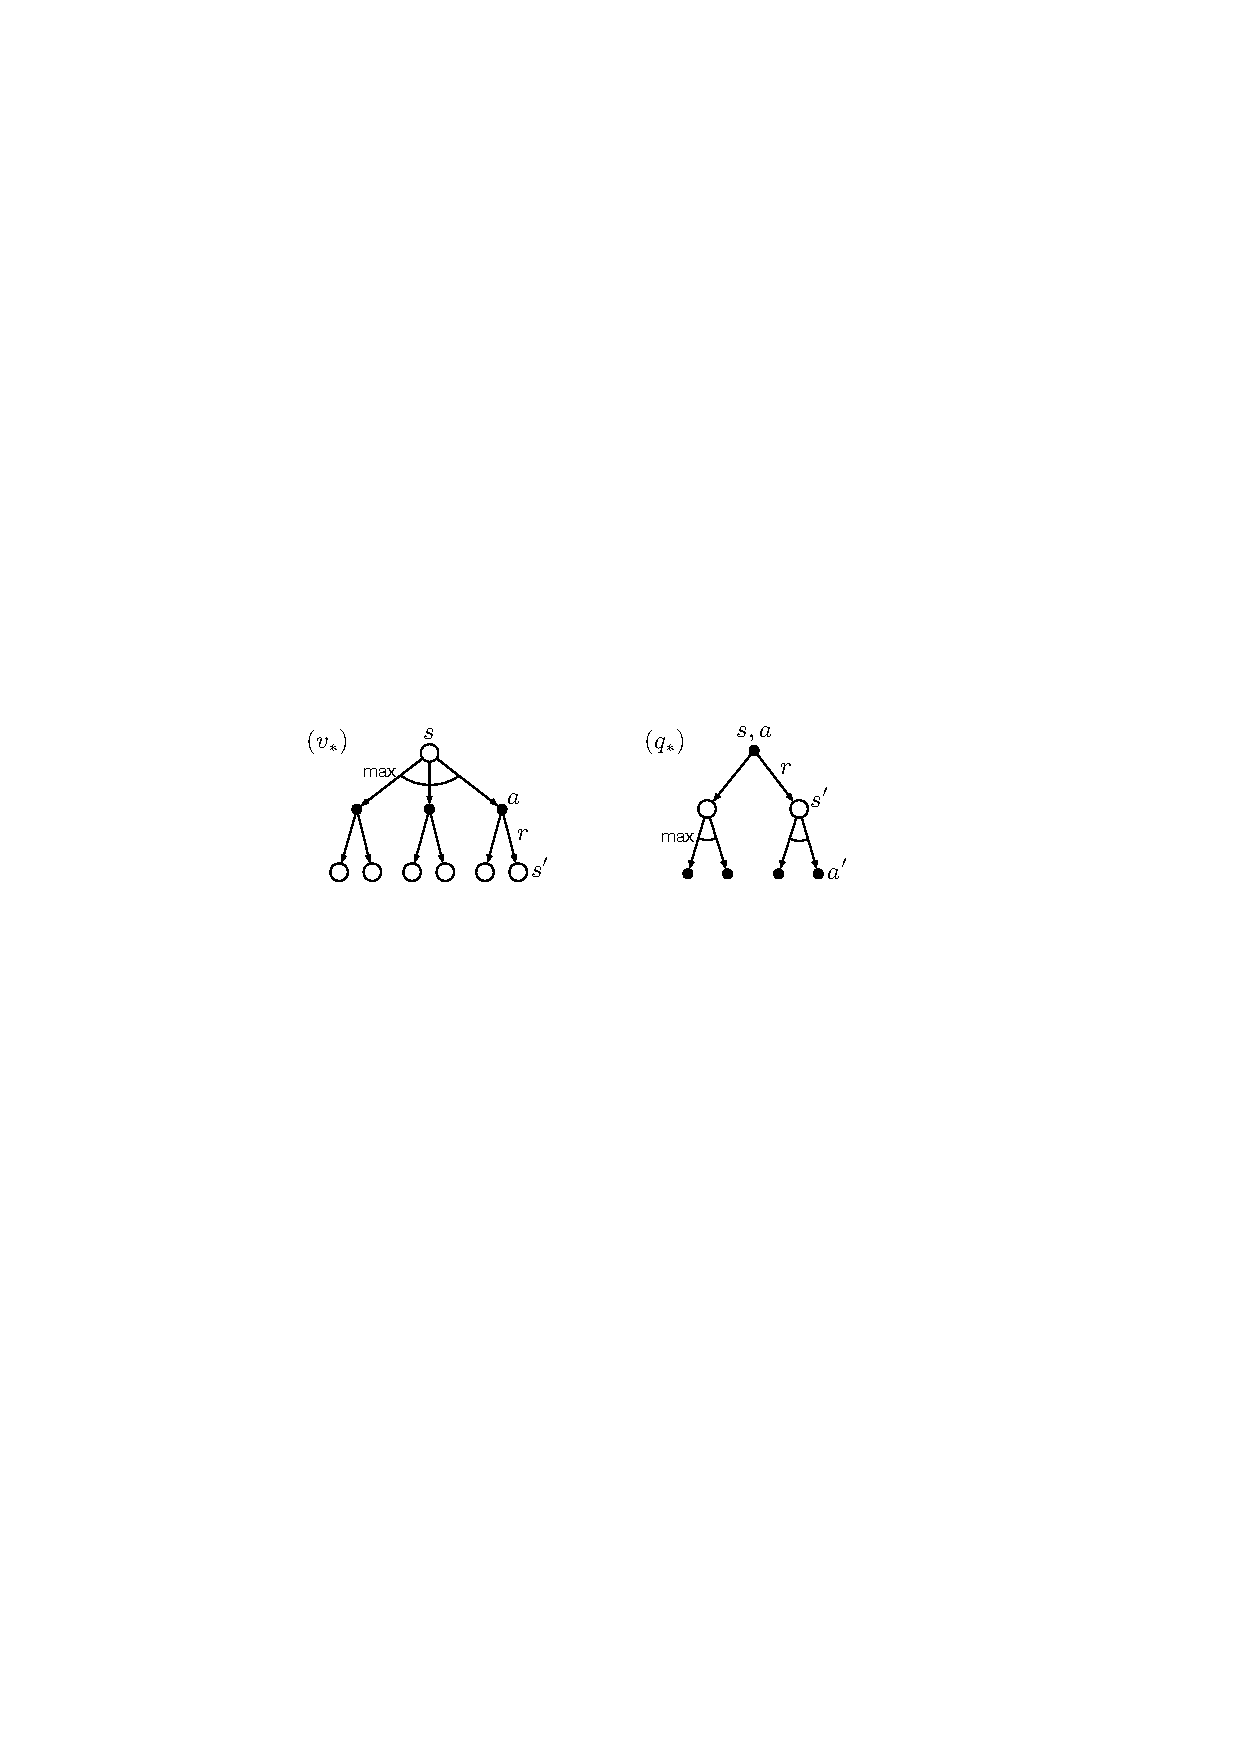
\includegraphics[width=\linewidth{}]{figures/backup.pdf}
  \caption{最適価値関数のバックアップ図 (文献\cite{Sutton1998}より引用) \label{fig:backup}}
\end{figure}

\subsection{価値ベースな手法}
状態$s$における最適方策に従った具体的な行動は$\argmax \mathbb{E}[R_{t+1} + \gamma v_*(S_{t+1}) | S_t=s, A_t=a]$と, $1$ステップ先の状態を探索してそれらの最適状態価値関数を参照することで計算できる.
最適行動価値関数が参照できれば, $1$ステップ先の状態を探索する必要すらなく, 単に$\argmax q_*(s, a)$を選択すればよい.
最適方策を得るために価値関数を学習する手法は価値ベースな手法と呼ばれる.

Q学習は最も基本的な価値ベースな手法の$1$つで, 最適行動価値関数$q_*$の推定値$Q$を得られた経験から学習する.
状態$S_t$から行動$A_t$を選択し, 報酬$R_{t+1}$を獲得して次の状態$S_{t+1}$に遷移したとする.
このときQ学習は以下の更新式~\ref{eq:q_learning}に従って$Q(S_t, A_t)$を更新する.
\begin{align}
  \label{eq:q_learning}
  Q(S_t, A_t) \leftarrow Q(S_t, A_t) + \alpha [R_{t+1} + \gamma \max_a Q(S_{t+1}, a) - Q(S_t, A_t)] 
\end{align}
式~\ref{eq:q_learning}は現在の推定値$Q(S_t, A_t)$を, ベルマン最適方程式~\ref{eq:bellman_q_opt}の右辺の推定値である$R_{t+1} + \gamma \max_a Q(S_{t+1}, a)$に近づけていると解釈できる.
任意の$(s, a) \in \mathcal{S} \times \mathcal{A}$について$Q(s,a)$が更新され続けるという条件の下で, Q学習は収束が保証されている.

状態集合や行動集合が大きい場合や有限でない場合には, テーブル形式でQ値を保持することができないため何らかの関数近似を行う必要がある.
近年では深層学習の研究の発展により, 関数近似の方法としてニューラルネットワークが用いられることが多い.
価値関数や方策をニューラルネットワークで近似する手法は, まとめて深層強化学習と呼ばれる.
Deep Q Network~(DQN)~\cite{DQN}は深層強化学習の先駆けとして有名な手法である. 
名前が示す通りDQNはQ値をニューラルネットワークで近似し手法である.
DQNの発表以降, 様々な工夫が提案され続けている.
詳細は文献~\cite{deepRL}の$4$節などを参照されたい.

\subsection{方策ベースな手法}

\section{AlphaZero}
Silverらが提案したAlphaZero~\cite{AlphaZero}は, 二人ゼロ和完全確定情報ゲームを対象とした有力な深層強化学習手法である.
囲碁, 将棋, チェスにおいて当時の有力なプログラムを上回る強さを示した.
AlphaZeroは盤面の特徴量を入力として方策と価値を出力するニューラルネットワークを, 自己対戦を通して得たデータから学習する.
自己対戦において, AlphaZeroはモンテカルロ木探索~(MCTS)~というアルゴリズムを使用して指し手を選択する.

\subsection{モンテカルロ木探索}
ここではAlphaZeroが使用したモンテカルロ木探索~(MCTS)~について説明する.
MCTSは探索で発見した各状態~(囲碁や将棋では盤面)~に対応するノードから成る探索木を構築する.
それぞれの状態と行動の対~$(s,a)$~について, ${N(s,a), W(s,a), Q(s,a), P(s,a)}$という$4$つの統計量を管理する.
\begin{itemize}
  \item $N(s,a) \cdots$探索中に$s$から$a$を選択した回数
  \item $W(s,a) \cdots$最適行動価値$q_*(s,a)$の推定値の累計
  \item $Q(s,a) \cdots$最適行動価値$q_*(s,a)$の推定値の平均~($W(s,a) / N(s,a)$)
  \item $P(s,a) \cdots$ニューラルネットワークが評価する$s$から$a$を選択する確率
\end{itemize}

探索木は最初, 現在の盤面に対応するノードである根ノードのみから成る.
MCTSは選択, 展開, 評価, 逆伝播の$4$つのステップを繰り返すことで, 良い手を選択するための探索手法である.
この$4$つのステップはまとめてシミュレーションと呼ばれる.
シミュレーションを繰り返すことで探索木は深くなり, 良い手を選択することができる.
以下ではそれぞれのステップについて説明する.

\subsubsection*{選択}
現在のゲーム木の根ノードから有望な子ノードを選択し, 葉ノードに至るまで辿り続ける.
ここで有望なノードとは暫定の評価の高さと
\begin{figure}
  \centering
  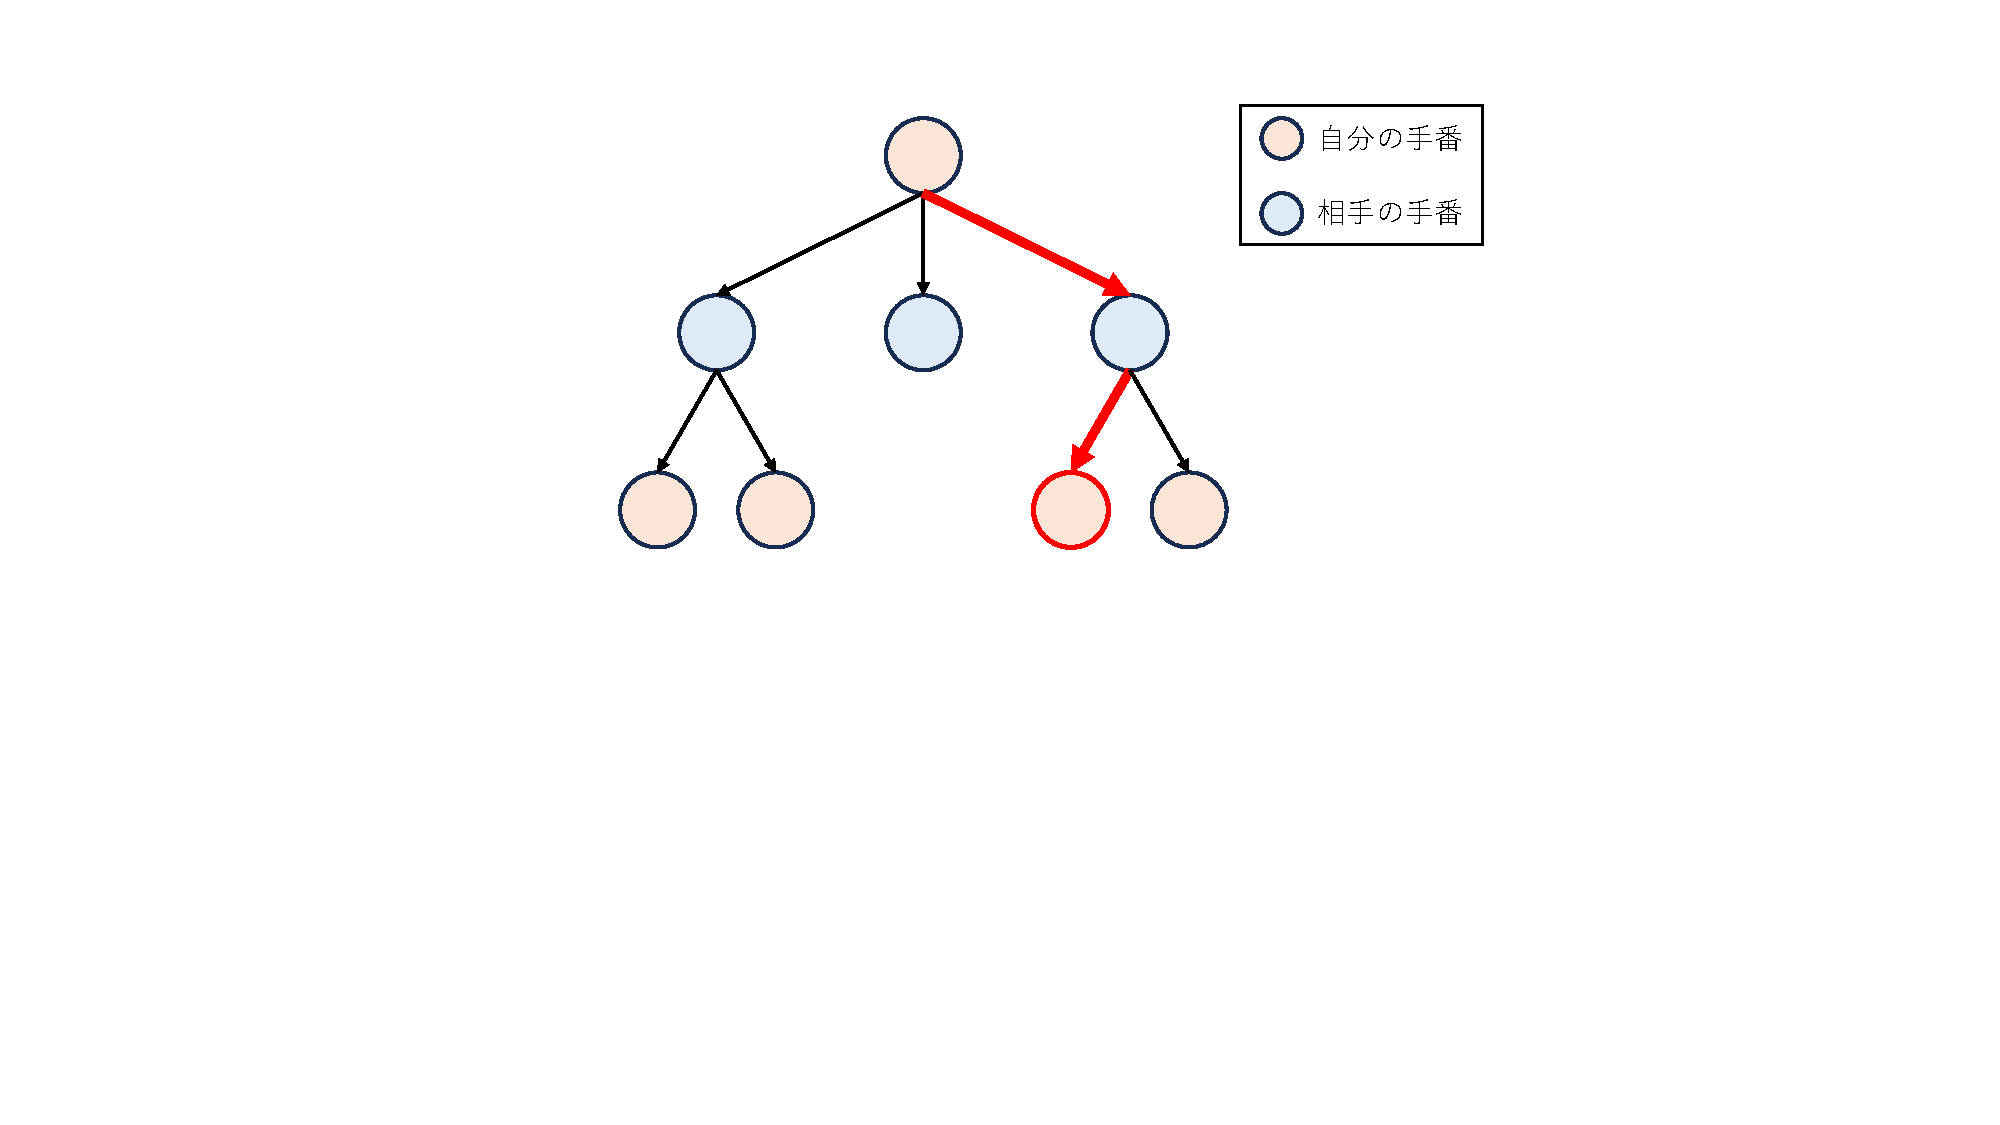
\includegraphics[width=\columnwidth]{figures/selection.pdf}
  \caption{選択}
  \label{fig:selection}
\end{figure}

\subsubsection*{展開}
\subsubsection*{評価}
\subsubsection*{逆伝播}

\subsection{ニューラルネットワークの学習}
MCTSの探索木における各ノードは
MCTSは選択, 展開, 評価, 逆伝播という$4$つのステップを繰り返すことで良い手を選ぶための手法である.

\section{2048への強化学習の応用}
\ref{sec:rl_general}節では強化学習一般の概要について説明した.
これを踏まえて本節では, 2048を対象とした強化学習研究の先行研究について概説する.
\begin{align}
  \label{eq:td_afterstate}
  Q(S_t, A_t) \leftarrow Q(S_t, A_t) + \alpha [R_{t+1} + \gamma \max_a Q(S_{t+1}, a) - Q(S_t, A_t)]
\end{align}


\subsection{TD afterstate学習}
Szubertら~\cite{Szubert}はTD afterstate学習と呼ばれる価値ベースの学習手法を提案した.
TD afterstate学習ではafterstateの価値
N-tupleネットワークは2048の盤面特徴量の
提案したTD afterstate学習は現在でも主流の手法の$1$つである.


\subsection{Afterstate PPO}

\subsection{Stochastic MuZero}
